% 1957 年全国卷第 4 题：四面体棱上四个中点。
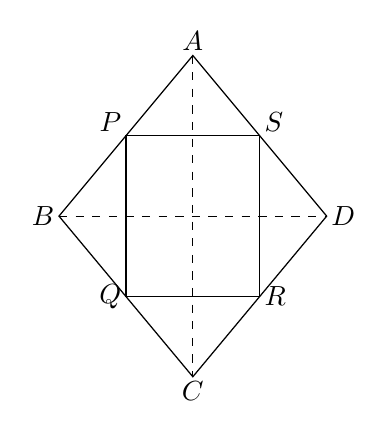
\begin{tikzpicture}[scale=0.85, line width=0.45pt,
  every node/.style={inner sep=1.5pt}]
  \coordinate (A) at (0,2.8);
  \coordinate (B) at (-2,0.4);
  \coordinate (C) at (0,-2.0);
  \coordinate (D) at (2,0.4);
  \coordinate (P) at (-1,1.6);
  \coordinate (Q) at (-1,-0.8);
  \coordinate (R) at (1,-0.8);
  \coordinate (S) at (1,1.6);
  \draw (A)--(B)--(C)--(D)--cycle;
  \draw[dashed] (B)--(D) (A)--(C);
  \draw (P)--(Q)--(R)--(S)--cycle;
  \node[anchor=south] at (A) {$A$};
  \node[anchor=east] at (B) {$B$};
  \node[anchor=north] at (C) {$C$};
  \node[anchor=west] at (D) {$D$};
  \node[anchor=south east] at (P) {$P$};
  \node[anchor=east] at (Q) {$Q$};
  \node[anchor=west] at (R) {$R$};
  \node[anchor=south west] at (S) {$S$};
\end{tikzpicture}
